\section{Maxwell 高阶补偿：比动态弱空间更具体的物理对象}
\label{sec:jets}

\subsection{A17 的有效连接与不能直接等同的部分}
以下正规方程使用同一个 anchor residual $r$ 与 $Hs=-h$ 的符号约定；若 anchor residual 同时改变，需另加相应变化项。
A17 最终理论把 current 子空间改变写成
\[
\Delta J=Y_C\Gamma_C^{-1}N_C,
\]
其中 $Y_C$ 是含 retained feedback 的接收返回，$N_C$ 是材料注入，$\Gamma_C$ 为 current Schur 矩阵。材料正规方程的变化同时包含
\[
\Delta H=J_0^*\Delta J+\Delta J^*J_0+\Delta J^*\Delta J,
\qquad
\Delta h=\Delta J^*r.
\]
于是
\[
s_{\rm new}-s_{\rm old}
=-H_{\rm new}^{-1}(\Delta h+\Delta Hs_{\rm old}).
\]
这解释了用户的直觉：\textbf{一个中间表示是否重要，取决于它怎样从材料接受变化、怎样经过耦合返回观测，以及这些变化怎样作用于指定任务。} 只看中间表示的直接可见性不够。\refe{A17}

但将 current 换成 decoder latent 后，不能无条件说“完全同一物理理论”。一般隐式中间状态 $\mathcal R(q,m)=0$ 在 $\mathcal R_q$ 可逆时有
\[
J=\mathcal O_m-\mathcal O_q\mathcal R_q^{-1}\mathcal R_m,
\]
这是共同的消元结构；一个显式 decoder $G$ 则只有链式法则 $D(F\circ G)=DF\,DG$，除非另建隐式耦合模型，否则没有新的 Maxwell feedback 回路。decoder 决定可实现材料集合及 prior；current 是物理状态或其数值表示。代数结构可以迁移，物理解释和概率测度不能混用。

还要区分两个“阶”：$(I-D_mG_D)^{-1}$ 已在一阶材料导数中包含所有内部多次散射；$D^2F,D^3F$ 是对材料扰动的二阶、三阶响应。多次散射的散射阶数，不等于材料 Taylor 阶数。

\subsection{离散 Maxwell 的可计算系数}
材料坐标为实数。本节的复观测均按实部、虚部堆叠，并用对应实噪声协方差白化；$A,b_n$、投影和补偿坐标因此属于实 Hilbert 空间。current 递推本身仍可用复数求解，不能将复最小二乘得到的复系数当成可行的实材料补偿。
先用 scalar TM/VIE 的精确离散状态说明。对每个源，
\[
j=D_m(e^{\rm inc}+G_Dj),\qquad
L_0=I-D_{m_0}G_D,\qquad E_0=e^{\rm inc}+G_Dj_0,
\]
观测为 $F(m)=Sj$。这里 $D_m$ 为对角材料乘子；所有源共享同一材料。假定 $L_0$ 可逆，并在声明局部域内保持非奇异。设
\[
m(h)=m_0+\sum_{n\ge1}h^nm_n,\qquad
j(h)=j_0+\sum_{n\ge1}h^nj_n .
\]
系数中不含阶乘；$m_n=m^{(n)}(0)/n!$。

\begin{theorem}[补偿后的 Maxwell 响应 jets]
\label{thm:jets}
在上述解析、可逆条件下，
\begin{equation}
L_0j_n
=
D_{m_n}E_0+
\sum_{k=1}^{n-1}D_{m_k}G_Dj_{n-k}.
\label{eq:jet-recurrence}
\end{equation}
令 $\Gamma=\sigma^2\Sigma$，固定噪声形状白化 $\bar F=\Sigma^{-1/2}F$，以免把 $\sigma$ 混入响应系数。选择预先声明的强材料坐标 $z\in\R^r$、弱坐标 $h$ 和可行解析浸入 chart $m=m(z,h)$；只讨论截至 $p$ 阶时，足够的 $C^{p+1}$ 正则性及余项控制即可。强坐标位于声明可行域的相对内点，要求补偿后的实际材料弧 $m'(0)\ne0$，并要求
\[
m(0,0)=m_0,\quad \partial_hm(0,0)\ne0,\quad
A=D_z\bar F(m(z,h))|_{0}
\]
满列秩。设 $P_A=A(A^*A)^{-1}A^*$。局部存在唯一的 $z(h)$ 满足
\begin{equation}
A^*\big[\bar F(m(z(h),h))-\bar F(m_0)\big]=0.
\label{eq:profile}
\end{equation}
按 $h$ 逐阶展开，若 $b_n$ 是已知低阶系数及本阶固定材料曲率产生的响应项，则
\begin{equation}
z_n=-A^+b_n,\qquad c_n=(I-P_A)b_n.
\label{eq:compensated-jets}
\end{equation}
首个非零 $c_p$ 是该声明 chart、强补偿类与指定材料弧上的首个剩余响应系数。
\end{theorem}
\begin{proof}
把材料与 current 级数代入
$j=D_m(e^{\rm inc}+G_Dj)$，收集 $h^n$ 项；$D_{m_0}G_Dj_n$ 移到左侧即得式 \eqref{eq:jet-recurrence}。对式 \eqref{eq:profile}，其关于 $z$ 的导数为 $A^*A$，可逆；隐函数定理给出局部 $z(h)$。第 $n$ 阶仅有未知本阶强系数的线性项 $Az_n$，其余均由已知低阶项与 chart 导数决定，故 $A^*(Az_n+b_n)=0$，得到式 \eqref{eq:compensated-jets}。
\end{proof}

这是 Lyapunov--Schmidt 式约化和 Maxwell current 展开的具体结合。任意阶 Maxwell 导数及扰动 current 递推已有明确先例，因此本报告不宣称首次得到高阶导数。\refl{L3,L10} 可争取的贡献是：正确去除表征效应后，补偿系数能否解释真实材料歧义，给出可用余项与任务精度规律，并改善同精度总成本。

\subsection{二阶、三阶的具体表达}
若先用局部 affine 材料 chart
\[
m(h)=m_0+hv+Uz_2h^2+Uz_3h^3+\cdots,\qquad D\bar F(m_0)v=0
\]
且 $A=D\bar F(m_0)U$，则
\[
j_1=L_0^{-1}D_vE_0,
\]
\[
b_2=\Sigma^{-1/2}S L_0^{-1}D_vG_Dj_1,\qquad
z_2=-A^+b_2,
\]
\[
j_2=L_0^{-1}\!\left(D_{Uz_2}E_0+D_vG_Dj_1\right),
\]
\[
b_3=\Sigma^{-1/2}S L_0^{-1}
\left(D_vG_Dj_2+D_{Uz_2}G_Dj_1\right),\qquad
z_3=-A^+b_3.
\]
非线性 prior chart 的固定二、三阶材料项必须加入 $m_n$；删掉它们等于改变可行材料模型。更一般的向量 Maxwell 或 DDA 中，$X(m)$ 可能为张量本构或非线性 polarizability，应先对实际 $X(m(h))$ 展开，再用相同系数匹配；不能把 VIE 的 $D_m$ 直接当作任意 DDA 的真实离散本构。

如果 $c_2=0$，只能继续算 $c_3$，不能根据数值底噪声称“无限阶不可辨识”；如果所有阶确为零且解析收敛，才可由解析性推出局部响应恒定。非解析的 $C^\infty$ 平坦函数是反例，有限阶计算不能证明所有阶为零。

\subsection{余项与真正复用同一 LU 的条件}
对给定材料增量 $\Delta m$，
\[
j(m_0+\Delta m)-j_0
=(I-T)^{-1}L_0^{-1}D_{\Delta m}E_0,
\qquad T=L_0^{-1}D_{\Delta m}G_D.
\]
若可验证 $\|T\|\le\rho<1$，截断 Neumann 展开的 current 余项满足
\[
\left\|
\Delta j-\sum_{k=0}^{K}T^kL_0^{-1}D_{\Delta m}E_0
\right\|
\le
\frac{\rho^{K+1}}{1-\rho}
\|L_0^{-1}D_{\Delta m}E_0\|.
\]
乘接收与白化算子范数可得到输出界。它控制的是给定 $\Delta m$ 的 resolvent 展开；若材料曲线本身也截断，还需追加材料 Taylor 余项与对应响应稳定性界。$\|T\|<1$ 是充分条件，不通过不代表路径不存在；近共振、非正规放大时该界可能太松。

对 $P$ 个源，每一阶递推通常需要 $P$ 个 RHS，复用同一 $L_0$ 分解；构造强基响应另有 tangent/adjoint 费用，验证有限端点需新的状态分解。不能把“无高阶张量”写成“无物理费用”。

\subsection{正则材料弧、条件补偿类和坐标不变性}
为了把高阶归因于物理，至少要求
\[
\|m'(0)\|_{W_M}=1.
\]
$G(h)=m_0+ah^3$ 使一阶 Jacobian 为零，但以材料弧长作参数后可能只是线性响应。这是 decoder 奇性，不是 Maxwell 三阶观测。

对 $h=\psi(t)$ 且 $\psi'(0)\ne0$ 的正则重参数化，首个非零阶不变，系数乘 $\psi'(0)^p$。对 $h=t^3$ 这样的奇异变换则不保阶。不同强变量集合、不同可行 chart、不同高阶弱弧可以产生不同 $p$；所以不能声称每个材料方向都有一个不依赖路径的全局“固有阶”。

在 regular 材料 stratum 且 $D\bar F$ 满列秩时，任一正则材料弧的严格首阶必为 1。R7 的重点应包括有限噪声的交叉尺度，而非强行寻找不存在的 exact kernel。

\subsection{小非零一阶与高阶的交叉尺度}
若投影后的响应满足可验证的两项比较
\[
\|r(h)\|\asymp \lambda|h|+c|h|^p,\qquad
\lambda,c>0,\ p>1,
\]
并排除两项强相消，则
\[
h_\times\asymp(\lambda/c)^{1/(p-1)},\qquad
\sigma_\times\asymp
\lambda^{p/(p-1)}c^{-1/(p-1)}.
\]
$\sigma\ll\sigma_\times$ 时局部宽度约 $\sigma/\lambda$；$\sigma\gg\sigma_\times$ 且仍在有效局部域时，约 $(\sigma/c)^{1/p}$。严格 rank 始终可能不变，但实验噪声下的材料不确定性机制改变。向量项相消时必须直接分析完整曲线，不能盲用标量加法。

更严格地，若 $r(h)=\sum_{n=1}^pc_nh^n+R_{p+1}(h)$ 且
$\|R_{p+1}(h)\|\le M|h|^{p+1}$，一个真正可用的 $p$ 阶主导区间需同时满足
\[
\sum_{n<p}\|c_n\||h|^n\le\theta_1\|c_p\||h|^p,\qquad
M|h|^{p+1}\le\theta_2\|c_p\||h|^p,\qquad
\theta_1+\theta_2<1.
\]
还要落在可行材料、隐函数与 resolvent 有效域内。这些上下限可能没有交集；三阶分析不能忽略二阶项。系数非零也须超过其数值误差，其中强补偿会受 $\|A^+\|$ 放大。不能把未解析出小系数写成 exact zero。

\subsection{新增采集破坏补偿：一个非平凡反例}
考虑真实材料坐标 $(z,h)$ 的两个解析观测
\[
f_1(z,h)=z+h^2,\qquad f_2(z,h)=z-h^2.
\]
每个单独观测都可用 $z=\mp h^2$ 保持不变。两次观测共享同一材料 $z$ 后，
\[
\min_z\big(|z+h^2|^2+|z-h^2|^2\big)=2h^4,
\]
最优 $z=0$，剩余响应为 $(h^2,-h^2)$。联合一阶 Jacobian 的 $h$ 列仍为零，但联合观测已有二阶约束；只辨别 $|h|$，仍不辨别符号。

这是解析反例，不是已执行 Maxwell 实验。它给 E2 一个直接目标：不同频率/照明需要的材料补偿是否互相冲突？若每次采集允许独立的 nuisance $z_1,z_2$，恢复结论消失。对独立新增观测，允许补偿集合相同则最小总残差不减；新信息来自共享材料约束，不能靠把两个 Jacobian 的 rank 各自报出来代替。

\begin{figure}[htbp]
\centering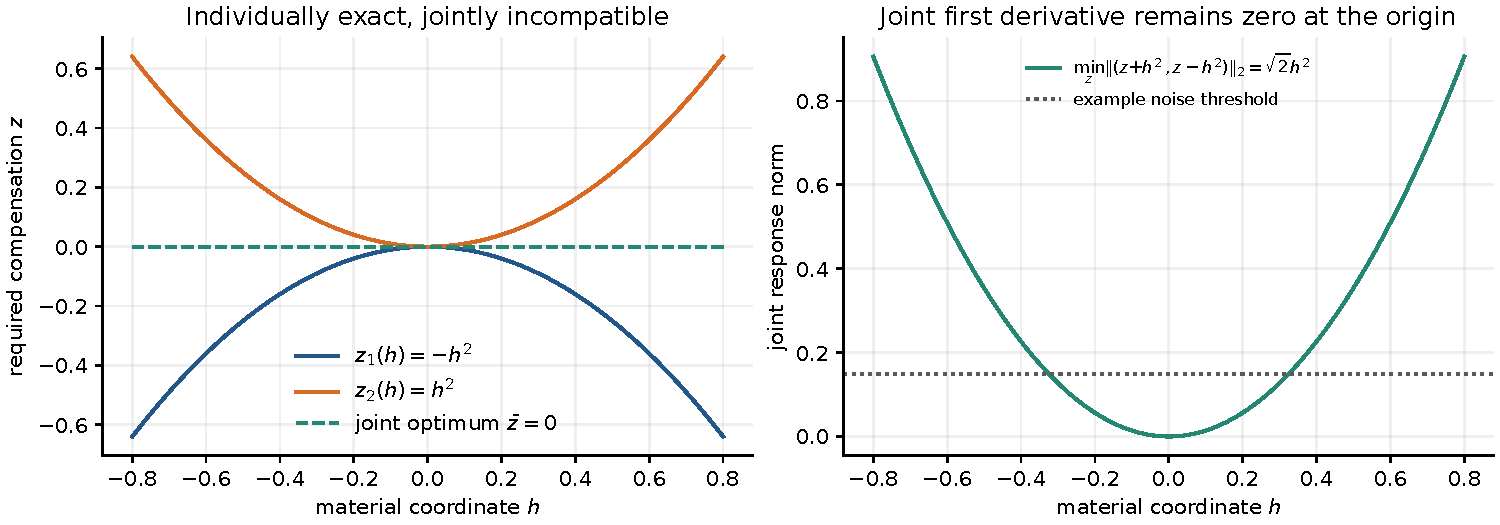
\includegraphics[width=\linewidth]{figures/shared_compensation.pdf}
\caption{共享补偿的解析反例。两个单独观测分别允许精确补偿，但同一材料不能同时采用两个相反的补偿。这不是 Maxwell 实验；它定义了 E2 要寻找或否证的物理机制。}
\end{figure}

\subsection{可计算的联合补偿分歧公式}
在某一阶 $n$，假定所有采集已共享相同的低阶材料系数，第 $a$ 个采集的本阶响应为 $A_a z+b_a$，且各 $A_a$ 满列秩。各采集按正确独立噪声块白化，使用同一物理强坐标 $z$；噪声相关时须先按联合协方差整体白化后重新建立分块。本阶强坐标可在声明内点无约束变化。定义
\[
H_a=A_a^*A_a,\qquad z_a=-A_a^+b_a,\qquad
c_a=(I-P_{A_a})b_a,\qquad
\bar z=\left(\sum_aH_a\right)^{-1}\sum_aH_az_a.
\]
则有精确分解
\begin{equation}
\min_z\sum_a\|A_az+b_a\|^2
=\sum_a\|c_a\|^2+\sum_a\|z_a-\bar z\|_{H_a}^2.
\label{eq:compensation-disagreement}
\end{equation}
证明只需写 $A_az+b_a=A_a(z-z_a)+c_a$，利用两项正交，再作加权平方完成。第一项是各采集本来就不可补偿的部分；第二项是它们要求的强材料补偿互相冲突产生的新约束。即使每个 $c_a=0$，第二项仍可为正。

这一加权最小二乘恒等式本身是成熟代数；多频、多照明共享同一材料也是成熟联合反演建模。可争取的新增贡献是最早冲突阶、有效材料位移区间和采集揭示能力的可计算预测。值得研究的 Maxwell 内容是 $b_a$ 由真实多次散射递推生成，并且所有采集必须共享同一材料补偿。式 \eqref{eq:compensation-disagreement} 可在未计算完整路径和 posterior 的情况下预测哪些新采集会破坏当前弱材料变化，是比“再做一次动态 SVD”更明确的候选物理机制。若不同采集早在更低阶就需要不同补偿，应在最早冲突阶应用，不能把各自独立走出的低阶路径混合。

\subsection{从几何到统计的局部下界}
若两材料 $m_0,m_h$ 的噪声形状白化响应距离 $d_h\le C|h|^p$，任务差异 $\Delta_\varphi\ge c|h|^s$，则 Gaussian 数据模型的 KL 为
\[
D_{\rm KL}(P_{m_h}\|P_{m_0})=\frac{d_h^2}{2\sigma^2}.
\]
取 $h=a\sigma^{1/p}$ 且 $a$ 足够小，可使总变差小于固定常数。由两点检验归约，任意任务估计器的这两个模型最大平方风险至少为
\[
\frac{\Delta_\varphi^2}{8}
\bigl(1-\|P_{m_h}-P_{m_0}\|_{\rm TV}\bigr)
\gtrsim \sigma^{2s/p}.
\]
证明是以估计值距两个任务值的最近者构造检验；分类错时平方误差至少 $\Delta_\varphi^2/4$，再用两模型平均检验错误下界。它是成熟 Le Cam 方法的条件应用，不是全局 Bayes 风险率。其作用是把已验证的 Maxwell 补偿弧转成任务无法任意准确的统计见证。

